%%%%%%%%%%%%%%%%%%%%%%%%%%%%%%%%%%%%%%%%%
% Beamer Presentation
% LaTeX Template
% Version 1.0 (10/11/12)
%
% This template has been downloaded from:
% http://www.LaTeXTemplates.com
%
% License:
% CC BY-NC-SA 3.0 (http://creativecommons.org/licenses/by-nc-sa/3.0/)
%
%%%%%%%%%%%%%%%%%%%%%%%%%%%%%%%%%%%%%%%%%

%----------------------------------------------------------------------------------------
%	PACKAGES AND THEMES
%----------------------------------------------------------------------------------------

\documentclass{beamer}

\mode<presentation> {

% The Beamer class comes with a number of default slide themes
% which change the colors and layouts of slides. Below this is a list
% of all the themes, uncomment each in turn to see what they look like.

%\usetheme{default}
%\usetheme{AnnArbor}
%\usetheme{Antibes}
%\usetheme{Bergen}
%\usetheme{Berkeley}
%\usetheme{Berlin}
%\usetheme{Boadilla}
%\usetheme{CambridgeUS}
%\usetheme{Copenhagen}
%\usetheme{Darmstadt}
%\usetheme{Dresden}
%\usetheme{Frankfurt}
%\usetheme{Goettingen}
%\usetheme{Hannover}
%\usetheme{Ilmenau}
%\usetheme{JuanLesPins}
%\usetheme{Luebeck}
%\usetheme{Madrid}
%\usetheme{Malmoe}
%\usetheme{Marburg}
%\usetheme{Montpellier}
\usetheme{PaloAlto}
%\usetheme{Pittsburgh}
%\usetheme{Rochester}
%\usetheme{Singapore}
%\usetheme{Szeged}
%\usetheme{Warsaw}

% As well as themes, the Beamer class has a number of color themes
% for any slide theme. Uncomment each of these in turn to see how it
% changes the colors of your current slide theme.

%\usecolortheme{albatross}
%\usecolortheme{beaver}
%\usecolortheme{beetle}
%\usecolortheme{crane}
%\usecolortheme{dolphin}
%\usecolortheme{dove}
%\usecolortheme{fly}
%\usecolortheme{lily}
\usecolortheme{orchid}
%\usecolortheme{rose}
%\usecolortheme{seagull}
%\usecolortheme{seahorse}
%\usecolortheme{whale}
%\usecolortheme{wolverine}

%\setbeamertemplate{footline} % To remove the footer line in all slides uncomment this line
%\setbeamertemplate{footline}[page number] % To replace the footer line in all slides with a simple slide count uncomment this line

%\setbeamertemplate{navigation symbols}{} % To remove the navigation symbols from the bottom of all slides uncomment this line
}

\usepackage{graphicx} % Allows including images
\usepackage{times,epsfig}
\usepackage{epstopdf}
\usepackage{booktabs} % Allows the use of \toprule, \midrule and \bottomrule in tables

%----------------------------------------------------------------------------------------
%	TITLE PAGE
%----------------------------------------------------------------------------------------

\title[Experimental Results]{Analysis of Networks} % The short title appears at the bottom of every slide, the full title is only on the title page

\author{Tao Wang} % Your name
\institute[Soton] % Your institution as it will appear on the bottom of every slide, may be shorthand to save space
{
University of Southampton \\ % Your institution for the title page
\medskip
\textit{t.wang@soton.ac.uk} % Your email address
}
\date{\today} % Date, can be changed to a custom date

\begin{document}

\begin{frame}
\titlepage % Print the title page as the first slide
\end{frame}

%\begin{frame}
%\frametitle{Overview} % Table of contents slide, comment this block out to remove it
%\tableofcontents % Throughout your presentation, if you choose to use \section{} and \subsection{} commands, these will automatically be printed on this slide as an overview of your presentation
%\end{frame}

%----------------------------------------------------------------------------------------
%	PRESENTATION SLIDES
%----------------------------------------------------------------------------------------

%------------------------------------------------
%\section{First Section} % Sections can be created in order to organize your presentation into discrete blocks, all sections and subsections are automatically printed in the table of contents as an overview of the talk
%%------------------------------------------------
%
%\subsection{Subsection Example} % A subsection can be created just before a set of slides with a common theme to further break down your presentation into chunks

\begin{frame}
\frametitle{Correlation of In and Out in Di-Graph}
\begin{figure}
\includegraphics[width=0.65\linewidth]{in_out.eps}
\end{figure}
\small{The Red points denote the correlation of in-degree and out-degree, and the Pearson correlation of in-degree and out-degree is 0.62. The blue points denote the correlation of in-strength (weights of link) and out-strength, and their Pearson correlation is 1.00, i.e., total positive correlation.}
\end{frame}

\begin{frame}
\frametitle{Correlation of Degree and Strength in Di-Graph}
\begin{figure}
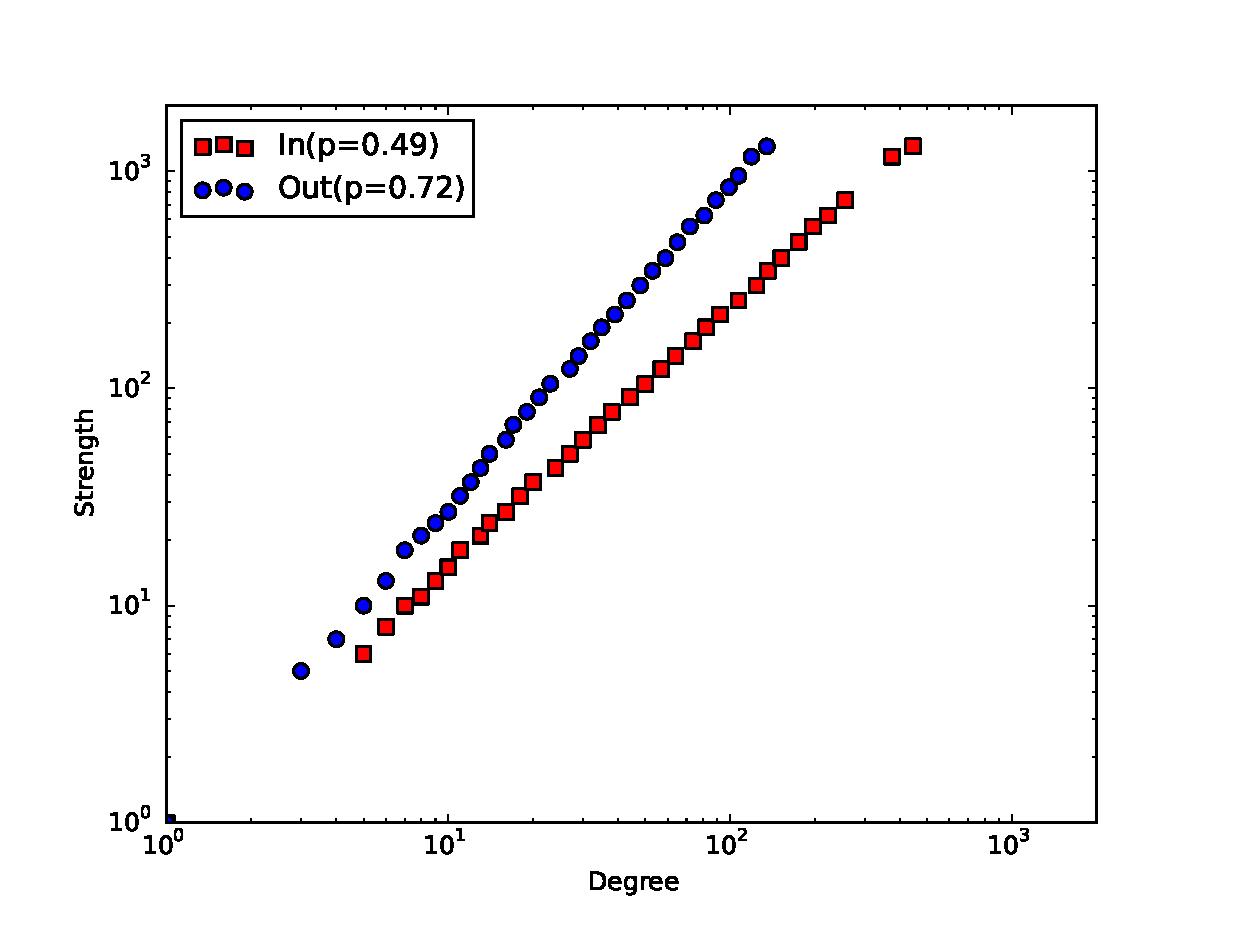
\includegraphics[width=0.65\linewidth]{de_st.eps}
\end{figure}
\small{The out frequencies(both degree and strength) are generally larger than the in ones. This confirms that the average number of friends of our friends are more than the number of friends that we have. We always focus on others, but they less focus on us.}
\end{frame}

\begin{frame}
\frametitle{Cumulative Probability Distribution in Di-Graph}
\begin{figure}
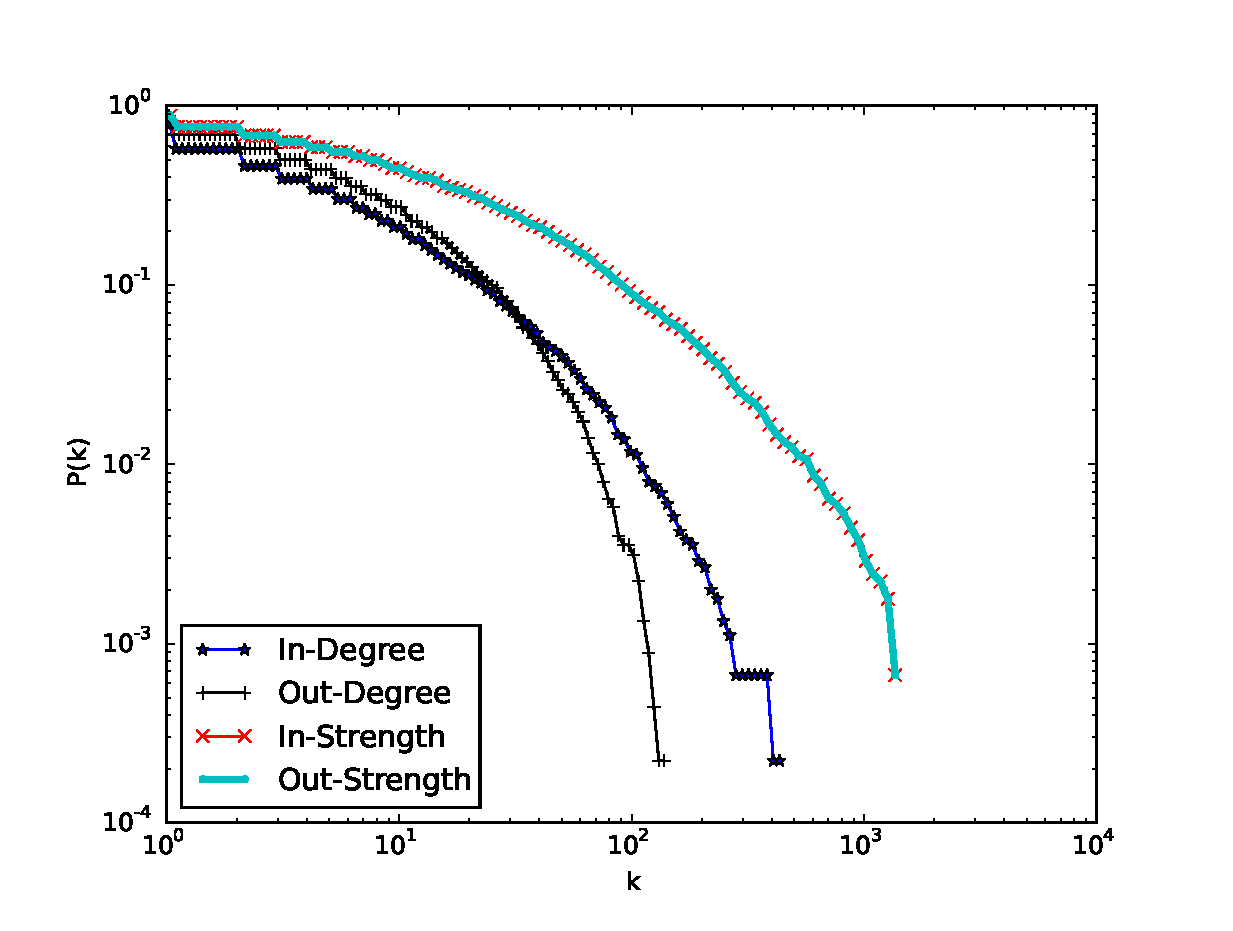
\includegraphics[width=.65\linewidth]{degree.eps}
\end{figure}
\small{As the in-strength is positive correlative to out-strength, their probability distributions are identical.}
\end{frame}

\begin{frame}
\frametitle{Correlation of Degree and Strength in UnDi-Graph}
\begin{figure}
\includegraphics[width=.65\linewidth]{undirect.eps}
\end{figure}
\small{The Pearson correlation of degree and strength in undirected graph is higher than those in directed graph(both in and out).}
\end{frame}


\begin{frame}
\frametitle{Cumulative Probability Distribution in UnDi-Graph}
\begin{figure}
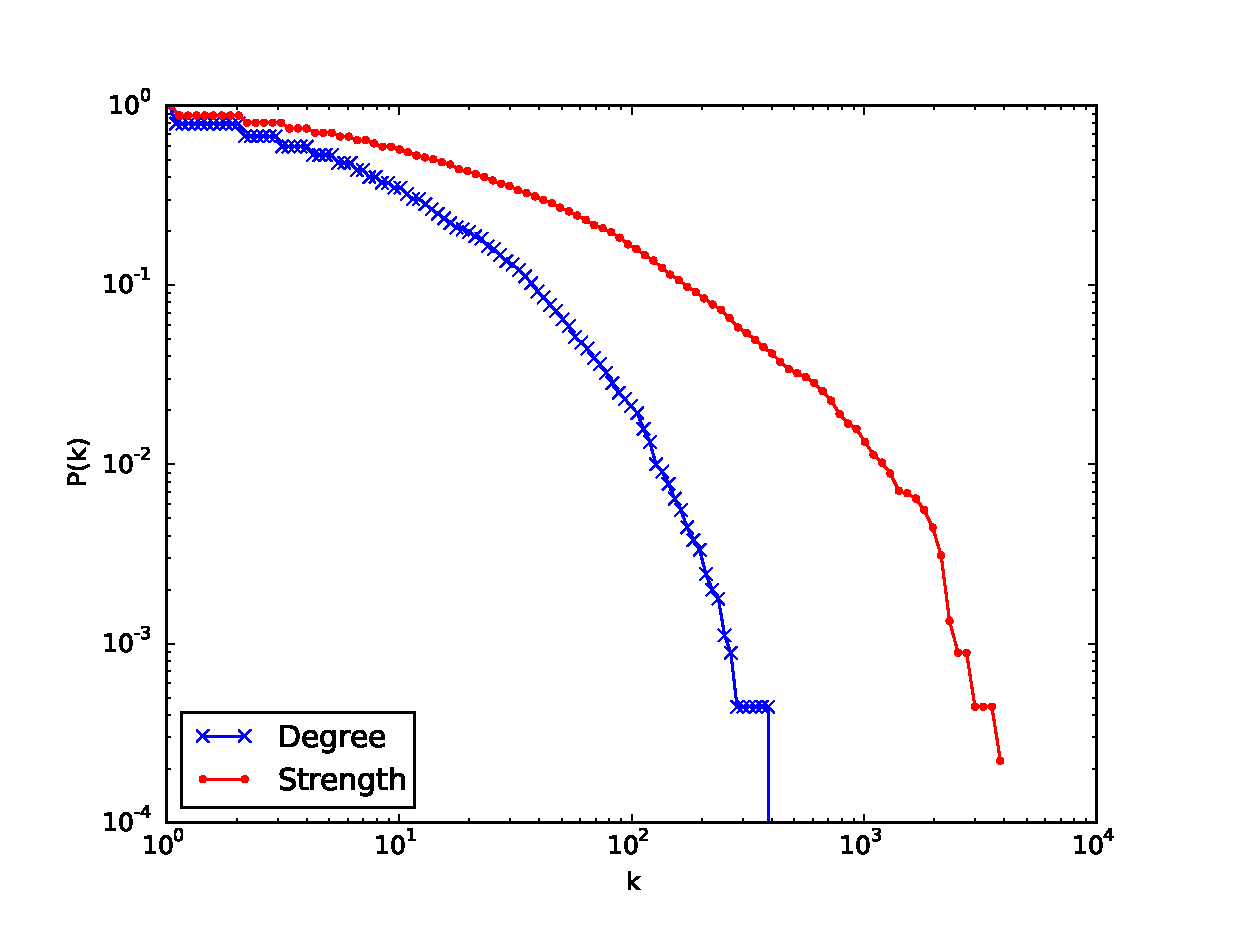
\includegraphics[width=.65\linewidth]{un_degree.eps}
\end{figure}
\small{The tail of strength distribution is long than that of degree.}
\end{frame}

\begin{frame}
\frametitle{Probability Distribution of Weights}
\begin{figure}
\includegraphics[width=.65\linewidth]{weight.eps}
\end{figure}

\small{Filtering users that have both GW and CW records, we can get 2,606 users from POI.csv. The ranges of global weights and current weights are in $[0.0, 1082.724104]$ and $[0.453592, 44741859695.9]$.}

\end{frame}

\begin{frame}
\frametitle{Cumulative Probability Distribution of Weights}
\begin{figure}
\includegraphics[width=.65\linewidth]{weight_cpd.eps}
\end{figure}
\small{The distributions of global weights and current weights are much similar. However, the current weights are generally larger than global weights, which seems users are getting fat.}

\end{frame}

%------------------------------------------------

\begin{frame}
\Huge{\centerline{The End}}
\end{frame}

%----------------------------------------------------------------------------------------

\end{document} 